\en{Let $ABC$ be a triangle such that $BC = CA$. Let $D$ be a point inside the segment $AB$ such that $AD<DB$. Let $P$ and $Q$ be two points inside the segments $BC$ and $CA$ respectively such that $\angle DPB = \angle DQA = 90^{\circ}$. Let the perpendicular bisector of $PQ$ intersect the segment $CQ$ at $E$. The circumcircles of $ABC$ and $PQC$ intersect at $C$ and $F$. Suppose that $P, E, F$ are collinear. Prove that $\angle ACB=90^\circ$.



\bigskip

\textbf{Solution (Horace):} Let $M$ be the midpoint of $AB$. then 
\[
\angle CMD = \angle CPD = 180^\circ - \angle CQD = 90^\circ,
\]
giving that $CPMDQ$ is an inscribed pentagon. Since $MCP=QCM$, $M$ lies on the perpendicular bisector of $PQ$.
Redifining $F$ as the intersection of $PE$ and the circumcenter of $PQC$, we see that $F$ is the reflection of $C$ through the perpendicular bisector fo $PQ$. Now for $FCAB$ to lie on a circle, the perpendicular bisector of $CF$, which is no different that the perpendicular bissector of $PQ$, should go through the circumcenter of $ABC$. This would give that $M$, as the intersection of the perpendicular bisector of $PQ$ and $AB$, should be the circumcenter of $ABC$. This is only possible if $\angle ACB=90^\circ$. \qedsymbol

\textbf{Solution (Matthew):}  The reflection of $C$ through the perpendicular bisector of $PQ$  clearly lies on the circumcircle of $PQC$. It also clearly lies on $PE$. In particular, this reflection must be $F$, giving us that $CPQF$ is an isoceles trapezoid. Therefore
\[
PF=CQ.
\]
Now
\[
\angle BFP= \angle BFC- \angle PFC = \angle BAC - \angle ACF = \angle ABC - \angle ABF = \angle FBP.
\]
So 
\[
BP=PF=CQ.
\]
Similarly (or from $AC=BC$) $CP=AQ$. This gives, using the similarity of $AQD$ and $BPD$,
\[
\frac{AD}{PC}=\frac{AD}{AQ}=\frac{DB}{PB}.
\]
Therefore $DP$ and $AC$ are parallel and $\angle ACB= 90^\circ$
\qedsymbol
\bigskip
\begin{center}
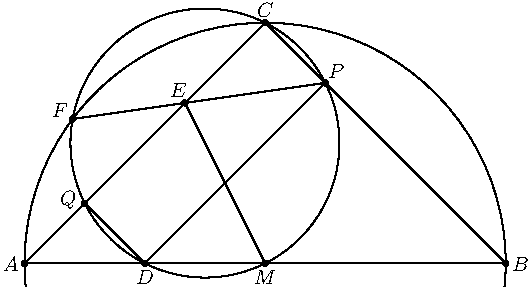
\includegraphics[scale=1.1]{2021/Selektion/muesterlosung/solutions/s8_fig.pdf}
\end{center}
\bigskip

\textbf{Marking Scheme (solution 1)}
General idea: an incomplete proof has a maximum of $5$ point. A complete proof with mistakes get 6 points.
\begin{enumerate}
\item 1P: Introducing $M$, in whatever meaningful definition (for example, circumcenter of $ABC$, midpoint of $AB$, intersection of $AB$ with the circumcircle of $PQC$, intersection of the perpendicular bisector of $CF$ with the angle bisector in $C$...). No points should be given for a letter on a drawing.
\item 1P: Finding that $CPDQ$ are cocyclic. This point is also given if the student prove points (c) or (d).
\item 2P: Finding that $CPMQ$ is an inscribed quadrilateral, or analogous statement depending on the definition of $M$. This point is also given if the student prove point (d).
\item 1P: Proving that the perpendicular bisector of $CF$ intersect $AB$ in its midpoint.
\item 2P: Finishing.
\end{enumerate}

\textbf{Marking Scheme (solution 2)}
\begin{enumerate}
\item 2P: Showing that $FPB$ or $AQF$ are isoceles. This point is also given if one shows that $BP=CQ$ or $AQ=CP$.
\item 2P: $BP=CQ$ or $AQ=CP$
\item 1P: Stating that $AQD$ and $BPD$ are similar.
\item 2P: Finishing.
\end{enumerate}
}